\documentclass[11pt,a4paper]{article}

% ===================== packages =====================
\usepackage[utf8]{inputenc}
\usepackage[T1]{fontenc}
\usepackage{lmodern}
\usepackage[a4paper,margin=2.5cm,headheight=46pt,headsep=14pt,footskip=34pt]{geometry}
\usepackage{amsmath,amssymb}
\usepackage{graphicx}
\usepackage{booktabs}
\usepackage{caption}
\usepackage{subcaption}
\usepackage{xcolor}
\usepackage{enumitem}
\usepackage{listings}
\usepackage{fancyhdr}
\usepackage{lastpage}
\usepackage{tikz}
\usepackage[hidelinks]{hyperref}

\graphicspath{{figures/}}
\newcommand{\degC}{\ensuremath{^{\circ}}C}

% ===================== Baltic-style colours =====================
\definecolor{baltic}{rgb}{0.10,0.20,0.42}   % navy for header text
\definecolor{codegray}{gray}{0.96}
\definecolor{codeblue}{rgb}{0.0,0.0,0.7}
\definecolor{codegreen}{rgb}{0.0,0.45,0.0}

% ===================== document metadata =====================
\newcommand{\DocTitleA}{Thermal Simulation of a Showerhead Injector}
\newcommand{\DocTitleB}{Operating with Hydrogen Peroxide}
\newcommand{\DocSubtitle}{3D Transient Heat-Up Analysis of an HTP-Cooled Injector Face Plate}
\newcommand{\DocAuthor}{Pawe\l{} Polanowski 333489}
\newcommand{\DocDate}{16.06.2026}

% ===================== faculty name (plain text) =====================
\newcommand{\facultyname}{Wydzia\l{} Mechaniczny Energetyki i Lotnictwa}

% ===================== headers / footers =====================
\pagestyle{fancy}
\fancyhf{}
\renewcommand{\headrulewidth}{0.6pt}
\renewcommand{\footrulewidth}{0.6pt}
\fancyhead[L]{\color{baltic}\small \DocTitleA\\ \DocTitleB}
\fancyhead[R]{\footnotesize\begin{tabular}{@{}r@{}}Wydzia\l{} Mechaniczny\\ Energetyki i Lotnictwa\end{tabular}}
\fancyfoot[L]{\small\MakeUppercase{\leftmark}}
\fancyfoot[R]{\small Date: \DocDate\\ Page \thepage{} of \pageref{LastPage}}

% leftmark = section number + name
\renewcommand{\sectionmark}[1]{\markboth{\thesection\quad #1}{}}

% ===================== listings style =====================
\lstset{
  basicstyle=\ttfamily\footnotesize,
  backgroundcolor=\color{codegray},
  keywordstyle=\color{codeblue}\bfseries,
  commentstyle=\color{codegreen}\itshape,
  stringstyle=\color{red!60!black},
  breaklines=true, frame=single, showstringspaces=false,
  inputencoding=utf8, extendedchars=true, tabsize=2, captionpos=b,
}

\begin{document}

% ============================================================
%  TITLE PAGE
% ============================================================
\thispagestyle{empty}
\begin{center}
  \vspace*{1.5cm}
  {\large\bfseries \facultyname}\\[2.2cm]
\end{center}

\noindent
\begin{minipage}[t]{0.55\textwidth}
  \begin{tabular}{@{}rl@{}}
    Edytor:      & \DocAuthor \\
    Data:        & \DocDate \\
    Ilo\'s\'c stron: & \pageref{LastPage} \\
  \end{tabular}
\end{minipage}%
\begin{minipage}[t]{0.45\textwidth}
  \begin{tabular}{@{}rl@{}}
    Autorzy: & \DocAuthor \\
  \end{tabular}
\end{minipage}

\vspace{2.5cm}
\begin{center}
  {\Huge\bfseries \DocTitleA\\[0.2em] \DocTitleB\par}
  \vspace{1.4cm}
  {\large \DocSubtitle\par}
  \vspace{0.4cm}
  {\large Modeling of Combustion Processes (MKWS)\par}
\end{center}

\vspace{1.2cm}
\begin{center}
\begin{minipage}{0.86\textwidth}
\small
This report describes the development of a three-dimensional transient thermal
simulation of a \emph{showerhead}-type rocket injector operating with high-test
hydrogen peroxide (HTP) as the oxidiser in a HTP\,/\,ethanol bipropellant
configuration. The objective is to predict the temperature distribution within
the injector face plate during combustion-chamber operation and to determine the
temperature at which a (quasi-)steady state is established. A unit-cell (sector)
model around a single injector orifice is solved with a fully three-dimensional
explicit finite-volume conduction scheme implemented in NumPy. The hot combustion
gases heat the chamber-side face by convection and radiation, while the liquid
HTP flowing through the orifices removes heat in a quasi-regenerative manner. The
simulation predicts a strongly non-uniform face temperature, from about
$393\,\degC$ at the cooled channel wall to about $849\,\degC$ in the metal between
orifices, with a heat-up time constant of approximately $1.0\,$s.
\end{minipage}
\end{center}

\clearpage

% ============================================================
%  CONTENTS
% ============================================================
\pagenumbering{roman}
\markboth{Contents}{}
\tableofcontents
\clearpage
\pagenumbering{arabic}

% ============================================================
\section{Introduction}
% ============================================================
Injector face plates in liquid rocket engines are exposed to extreme thermal
loads: the chamber side is heated by hot combustion gases, while the propellant
manifold and the internal flow passages are bathed in relatively cold liquid
propellant. The balance between gas-side heating and propellant-side cooling
sets the operating temperature of the plate, which is critical both for its
structural integrity and for the integrity of the propellant itself~\cite{huzel}.

This project develops an internal thermal simulator for a \emph{showerhead}
injector running on \textbf{hydrogen peroxide (HTP)} used as the oxidiser, with
ethanol as the fuel. In contrast to a one-dimensional through-thickness estimate,
a fully three-dimensional model is built so that the heat flow around the
individual cooling orifices -- and therefore the in-plane temperature
non-uniformity of the face -- is resolved.

\subsection{Project Objectives}
\begin{itemize}[noitemsep]
  \item Build a 3D transient conduction model of a showerhead injector unit cell.
  \item Represent the combined gas-side convective/radiative heating and the
        quasi-regenerative cooling by the HTP flowing through the orifices.
  \item Determine the steady-state temperature field and the heat-up time
        constant of the plate.
  \item Provide a parametric, dependency-light implementation (NumPy only) with
        reproducible figures and an animation of the heat-up.
\end{itemize}

% ============================================================
\section{Injector and Operating Case}
% ============================================================
\subsection{Showerhead Injector Concept}
A showerhead injector introduces the propellants through a regular pattern of
straight axial orifices drilled in a face plate. The plate considered here has
$n_\mathrm{holes}=60$ orifices distributed over a face of radius $R$. Because the
thermal boundary conditions are essentially uniform over the face, the plate is
geometrically periodic and can be represented by a single repeating
\textbf{unit cell} (sector) surrounding one orifice. The in-plane footprint per
orifice equals $A_\mathrm{face}/n_\mathrm{holes}$, which defines the cell pitch
\begin{equation}
  p = \sqrt{\frac{A_\mathrm{face}}{n_\mathrm{holes}}}
    = \sqrt{\frac{\pi R^2}{n_\mathrm{holes}}}.
  \label{eq:pitch}
\end{equation}

\subsection{Propellant Combination}
The engine uses high-test hydrogen peroxide as the oxidiser and ethanol as the
fuel -- a \emph{green}, storable combination that avoids the toxic hydrazine /
nitrogen-tetroxide propellants of earlier manoeuvring engines~\cite{ventura}.
For the present heat-transfer study the relevant data are the liquid HTP
properties (used to size the channel cooling) and the combustion-gas recovery
temperature (used as the hot-side driving temperature). The HTP\,/\,ethanol flame
temperature is taken as $T_\mathrm{gas}=2500\,$K.

\subsection{Thermal Loading Scenario}
During steady chamber operation the plate experiences:
\begin{itemize}[noitemsep]
  \item gas-side heating of the chamber face ($z=0$) by convection and radiation;
  \item internal cooling of each orifice wall by the through-flowing liquid HTP;
  \item cooling of the manifold face ($z=L$) by the cold inlet HTP.
\end{itemize}
The lateral faces of the unit cell are adiabatic, representing the mirror
symmetry between neighbouring orifices.

% ============================================================
\section{Computational Model}
% ============================================================
\subsection{Heat Conduction Equation}
Within the solid metal the temperature $T(\mathbf{x},t)$ obeys the transient
heat-conduction equation
\begin{equation}
  \rho\,c_p\,\frac{\partial T}{\partial t}
  = k\,\nabla^2 T
  = k\!\left(\frac{\partial^2 T}{\partial x^2}
            +\frac{\partial^2 T}{\partial y^2}
            +\frac{\partial^2 T}{\partial z^2}\right),
  \label{eq:heat}
\end{equation}
with density $\rho$, specific heat $c_p$ and conductivity $k$; the thermal
diffusivity is $\alpha=k/(\rho c_p)$.

\subsection{Gas-Side Boundary Condition}
The chamber-side face receives a combined convective and radiative flux
\begin{equation}
  q_\mathrm{gas}'' = h_\mathrm{gas}\,(T_\mathrm{gas}-T)
    + \varepsilon\,\sigma\,(T_\mathrm{gas}^4 - T^4),
  \label{eq:gas}
\end{equation}
with $\sigma=5.67\times10^{-8}\,\mathrm{W\,m^{-2}K^{-4}}$. The film coefficient
$h_\mathrm{gas}$ is the dominant uncertainty and is treated as an input
parameter.

\subsection{Channel Cooling -- Dittus--Boelter}
The convective coefficient inside an orifice is obtained from the
Dittus--Boelter correlation for a fluid being heated in turbulent pipe
flow~\cite{incropera}:
\begin{equation}
  \mathrm{Nu} = 0.023\,\mathrm{Re}^{0.8}\,\mathrm{Pr}^{0.4},
  \qquad
  h_p = \frac{\mathrm{Nu}\,k_\mathrm{prop}}{d_\mathrm{hole}},
  \label{eq:db}
\end{equation}
with $\mathrm{Re}=\rho_\mathrm{prop}\,v\,d_\mathrm{hole}/\mu$ and
$\mathrm{Pr}=c_{p,\mathrm{prop}}\,\mu/k_\mathrm{prop}$. The orifice wall flux is
$q_\mathrm{ch}'' = h_p\,(T - T_\mathrm{prop})$ and the manifold face is cooled by
$q_\mathrm{back}'' = h_\mathrm{back}\,(T - T_\mathrm{prop})$.

\subsection{Numerical Scheme and Stability}
Equation~\eqref{eq:heat} is discretised with a cell-centred finite-volume scheme
on a uniform Cartesian grid $N_x\times N_y\times N_z$; the cylindrical orifice is
a ``void'' region cut from the mesh (staircase approximation) whose faces carry
the convective flux instead of conduction. Time integration uses the explicit
forward-time, centred-space (FTCS) scheme, which is conditionally stable with the
step
\begin{equation}
  \Delta t = \frac{\mathrm{SF}}
  {2\alpha\!\left(\dfrac{1}{\Delta x^2}+\dfrac{1}{\Delta y^2}+\dfrac{1}{\Delta z^2}\right)
   + \dfrac{(h_\mathrm{gas}+h_\mathrm{back})A_z + 2h_p(A_x+A_y)
            + 4\varepsilon\sigma T_\mathrm{gas}^3 A_z}{\rho c_p V}},
  \label{eq:dt}
\end{equation}
with a safety factor $\mathrm{SF}=0.5$. A (quasi-)steady state is detected when
$\max|\Delta T/\Delta t| < 5\times10^{-3}\,\mathrm{K/s}$, and the heat-up time
constant $\tau$ is the time to reach $63.2\%$ of the total temperature rise of
the hottest probe.

\subsection{Material and Propellant Properties}
The baseline plate is 316L stainless steel; the cooling HTP is taken at
$\sim$90\,\% concentration. The properties are listed in Table~\ref{tab:props}.

\begin{table}[h]
\centering
\caption{Solid (316L) and liquid HTP properties used in the simulation.}
\label{tab:props}
\begin{tabular}{llr@{ }l}
\toprule
Quantity & Symbol & \multicolumn{2}{c}{Value} \\
\midrule
Plate conductivity    & $k$              & 16.0 & W\,m$^{-1}$K$^{-1}$ \\
Plate density         & $\rho$           & 8000 & kg\,m$^{-3}$ \\
Plate specific heat   & $c_p$            & 500  & J\,kg$^{-1}$K$^{-1}$ \\
Plate diffusivity     & $\alpha$         & $4.0\times10^{-6}$ & m$^2$\,s$^{-1}$ \\
HTP density           & $\rho_\mathrm{prop}$  & 1390 & kg\,m$^{-3}$ \\
HTP specific heat     & $c_{p,\mathrm{prop}}$ & 2730 & J\,kg$^{-1}$K$^{-1}$ \\
HTP conductivity      & $k_\mathrm{prop}$ & 0.50 & W\,m$^{-1}$K$^{-1}$ \\
HTP viscosity         & $\mu$            & $1.1\times10^{-3}$ & Pa\,s \\
HTP Prandtl number    & $\mathrm{Pr}$    & 6.01 & -- \\
HTP inlet temperature & $T_\mathrm{in}$  & 20   & \degC \\
\bottomrule
\end{tabular}
\end{table}

% ============================================================
\section{Implementation}
% ============================================================
\subsection{Solver Architecture}
The simulator is a single Python~3 program depending only on NumPy and
Matplotlib (no SciPy). The temperature field is stored as a 3D array; the solid
metal and the orifice void are distinguished by a boolean mask. All face fluxes
(conduction, channel convection, gas-side and manifold boundary terms) are
evaluated with vectorised array slicing, so one explicit time step is a handful
of NumPy operations.

\subsection{Unit-Cell Update}
Listing~\ref{lst:step} shows the core of the explicit update for the conduction
and channel-wall convection in the $x$-direction; the $y$- and $z$-directions are
analogous.

\begin{lstlisting}[language=Python,caption={Vectorised flux assembly (excerpt).},label={lst:step}]
# conduction between adjacent solid cells (x-direction)
both = solid[:-1] & solid[1:]
fc = np.where(both, Gx * (T[1:] - T[:-1]), 0.0)
Q[:-1] += fc; Q[1:] -= fc
# channel wall: solid cell facing the void (HTP) -> convective cooling
lsv = solid[:-1] & ~solid[1:]
Q[:-1] += np.where(lsv, Hx * (T_prop - T[:-1]), 0.0)
rsv = ~solid[:-1] & solid[1:]
Q[1:]  += np.where(rsv, Hx * (T_prop - T[1:]), 0.0)
# explicit time advance of the solid cells
Tn = T + (dt / Cap) * Q
Tn[~solid] = T_prop
\end{lstlisting}

\subsection{Simulation Configuration}
The gas-side, operating and geometric parameters of the baseline run are given in
Table~\ref{tab:config}.

\begin{table}[h]
\centering
\caption{Baseline simulation configuration.}
\label{tab:config}
\begin{tabular}{llr@{ }l}
\toprule
Quantity & Symbol & \multicolumn{2}{c}{Value} \\
\midrule
Flame / recovery temperature (HTP+ethanol) & $T_\mathrm{gas}$ & 2500 & K \\
Gas-side film coefficient & $h_\mathrm{gas}$ & 2000 & W\,m$^{-2}$K$^{-1}$ \\
Emissivity                & $\varepsilon$    & 0.30 & -- \\
Manifold cooling coeff.   & $h_\mathrm{back}$ & 1500 & W\,m$^{-2}$K$^{-1}$ \\
Total HTP mass flow       & $\dot m$         & 0.5  & kg\,s$^{-1}$ \\
Plate radius              & $R$              & 30   & mm \\
Plate thickness           & $L$              & 12   & mm \\
Number of orifices        & $n_\mathrm{holes}$ & 60 & -- \\
Orifice diameter          & $d_\mathrm{hole}$  & 1.5 & mm \\
Cell pitch (Eq.~\ref{eq:pitch}) & $p$        & 6.86 & mm \\
Grid                      & $N_x\!\times\!N_y\!\times\!N_z$ & \multicolumn{2}{l}{$26\times26\times22$} \\
Time step                 & $\Delta t$       & 1.54 & ms \\
\bottomrule
\end{tabular}
\end{table}

\subsection{Reproducibility}
The full simulation, post-processing and visualisation run with a single command,
\texttt{python3 injector\_thermal\_sim.py}, producing the figures used in this
report and an animated GIF of the heat-up. A $10\,$s transient completes in about
$25\,$s on a laptop.

% ============================================================
\section{Simulation Results}
% ============================================================
\subsection{3D Temperature Field}
Figure~\ref{fig:3d} shows the evolution of the unit-cell temperature field,
displayed as a cut-away around the cooling channel (gas side on top). The plate
heats from a uniform cold start to a state with a hot gas-side face and a cold
manifold side. The full animation is provided as the supplementary file
\texttt{injector\_thermal\_3d.gif}.

\begin{figure}[h]
\centering
\begin{subfigure}{0.32\textwidth}
  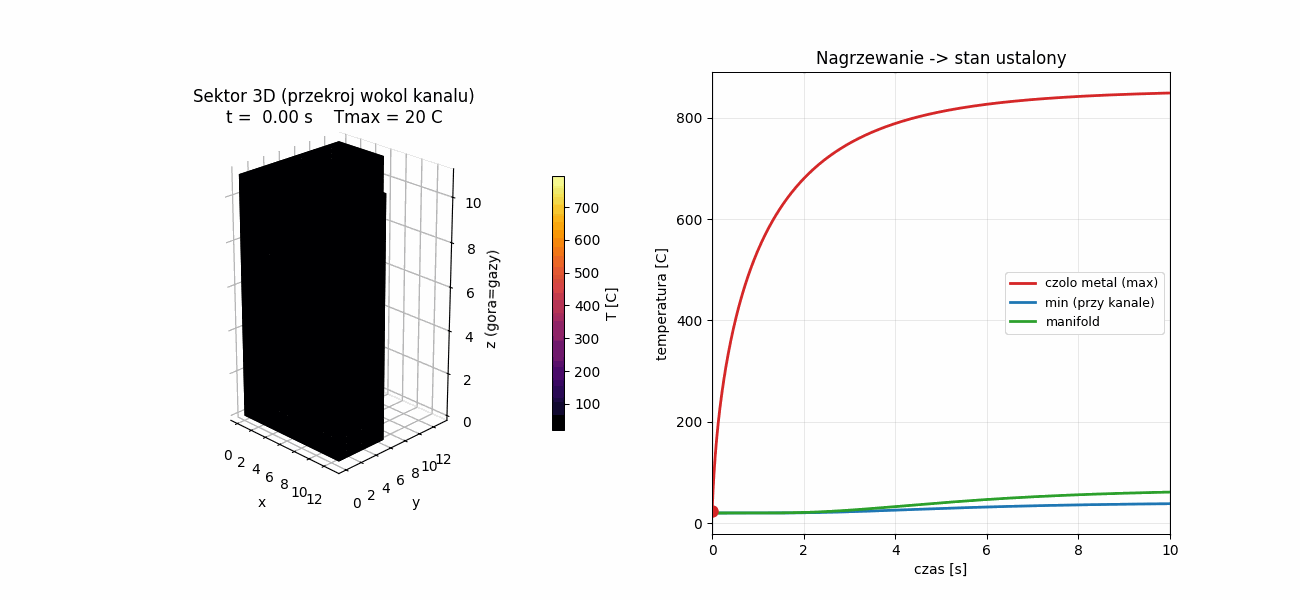
\includegraphics[width=\linewidth]{frame_start.png}
  \caption{$t=0$ (cold start)}
\end{subfigure}\hfill
\begin{subfigure}{0.32\textwidth}
  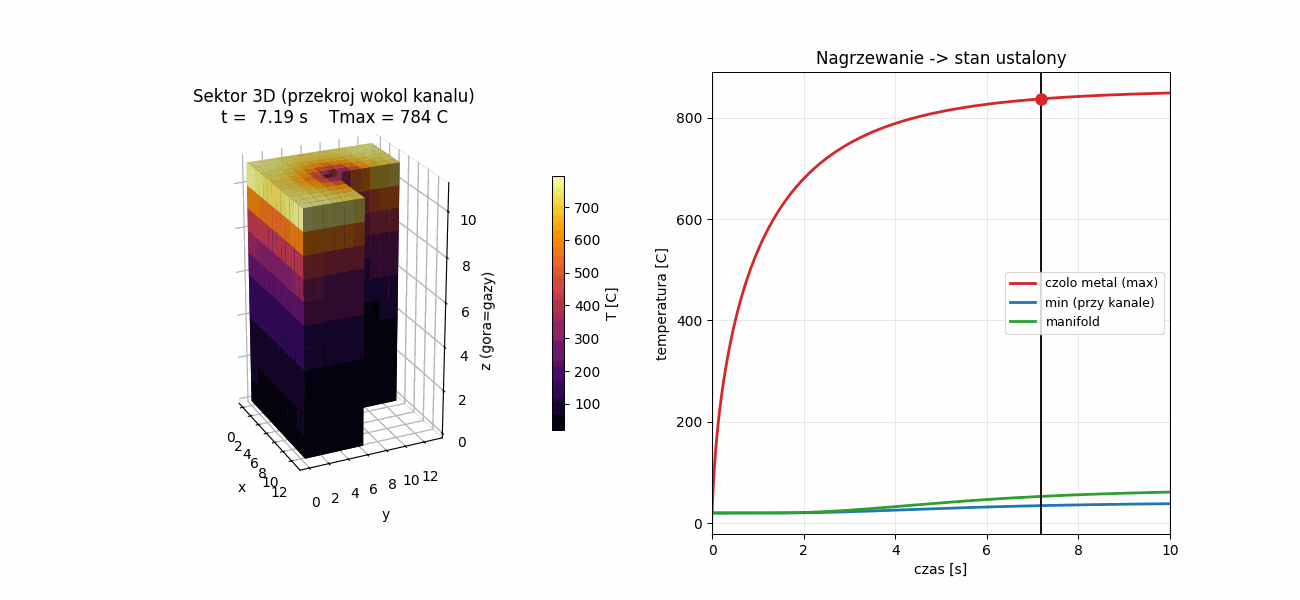
\includegraphics[width=\linewidth]{frame_mid.png}
  \caption{intermediate heat-up}
\end{subfigure}\hfill
\begin{subfigure}{0.32\textwidth}
  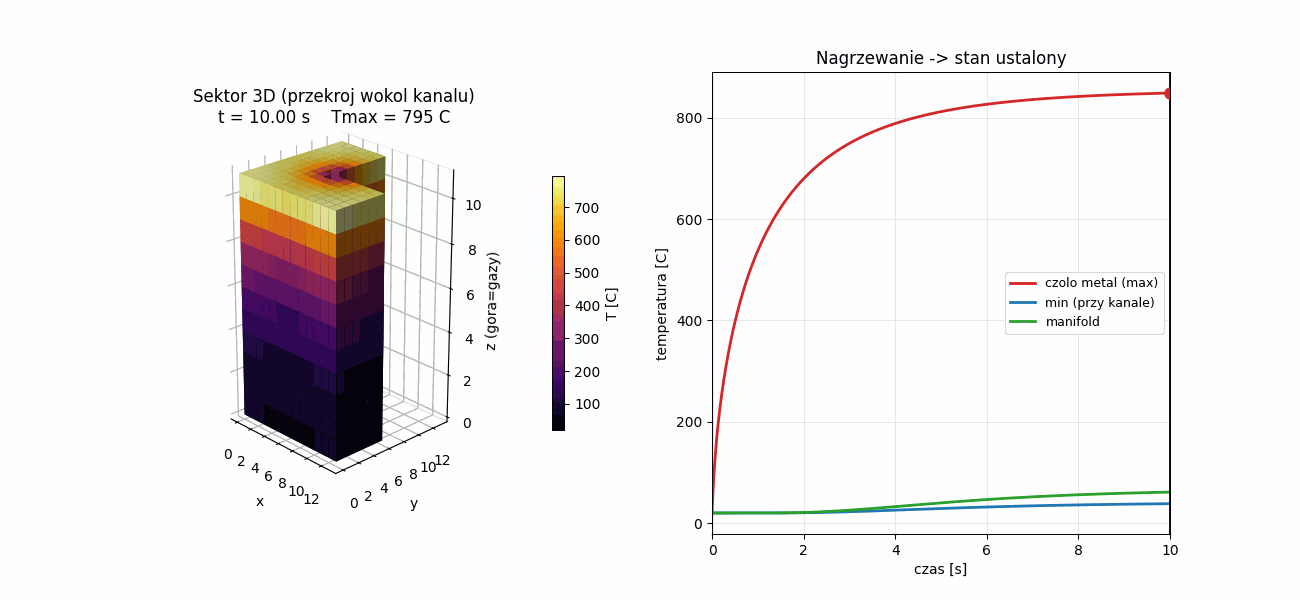
\includegraphics[width=\linewidth]{frame_steady.png}
  \caption{near steady state}
\end{subfigure}
\caption{Three-dimensional unit-cell temperature field at three instants
(cut-away around the orifice).}
\label{fig:3d}
\end{figure}

\subsection{Gas-Side Face Distribution}
The most important result is the strongly non-uniform face temperature
(Fig.~\ref{fig:face}): the metal adjacent to the cooled channel wall stabilises
near $393\,\degC$, whereas the metal midway between orifices reaches
$849\,\degC$, a difference of about $457\,$K across a single pitch. This in-plane
gradient is exactly the three-dimensional effect that motivates resolving the
orifice geometry.

\begin{figure}[h]
\centering
\begin{subfigure}{0.48\textwidth}
  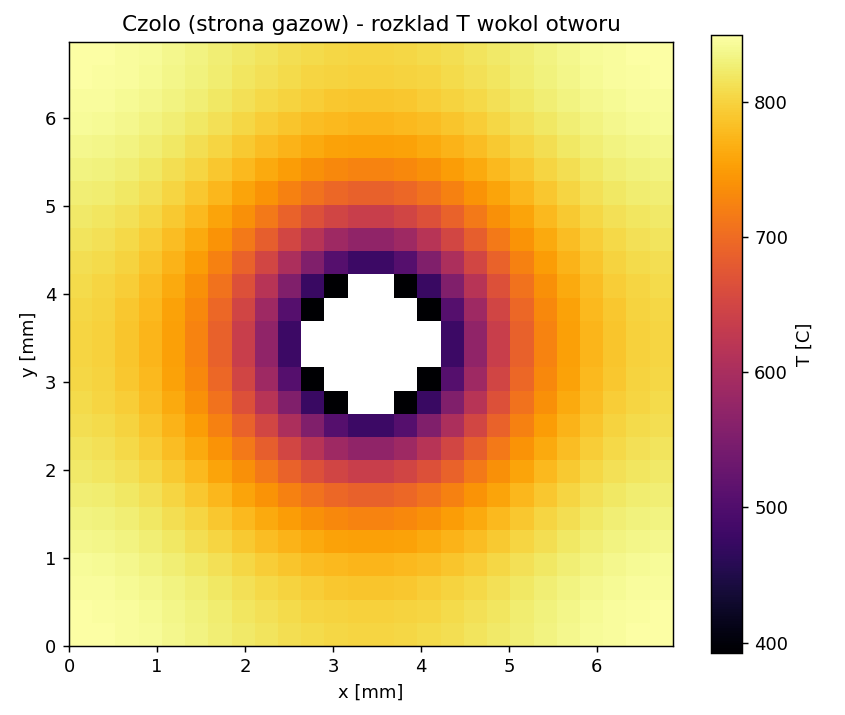
\includegraphics[width=\linewidth]{injector_thermal_face.png}
  \caption{Gas-side face: distribution around the orifice.}
  \label{fig:face}
\end{subfigure}\hfill
\begin{subfigure}{0.48\textwidth}
  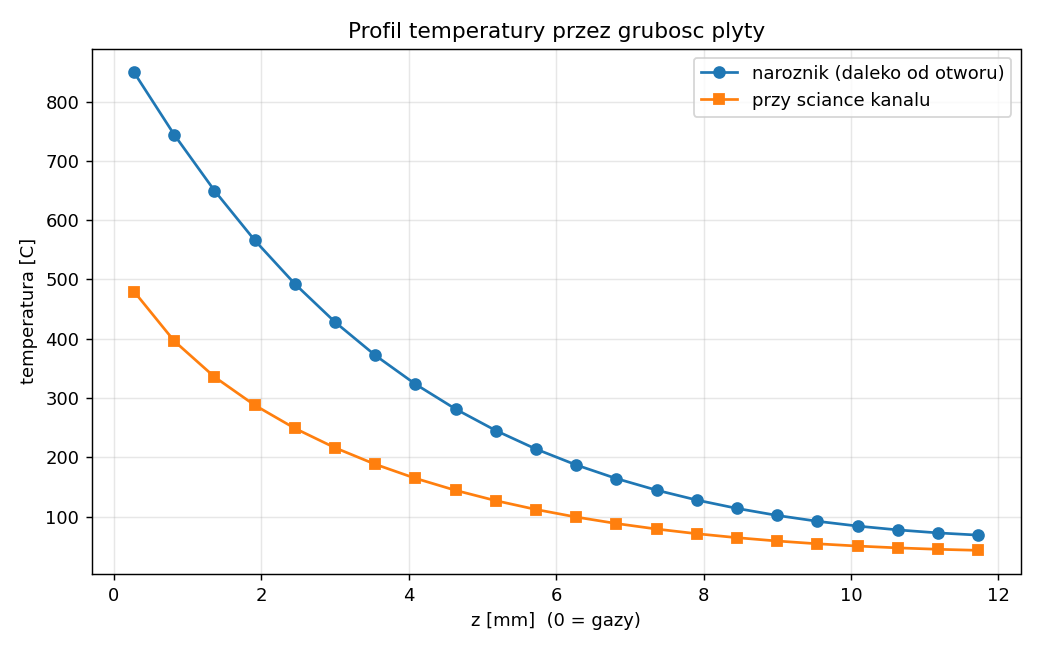
\includegraphics[width=\linewidth]{injector_thermal_profile.png}
  \caption{Through-thickness profiles.}
  \label{fig:profile}
\end{subfigure}
\caption{Steady-state temperature map of the gas-side face and through-thickness
profiles at the corner (far from the orifice) and next to the channel wall.}
\end{figure}

\subsection{Transient Behaviour and Time Constant}
Figure~\ref{fig:transient} shows the temperature histories of the characteristic
probes. The hot face responds quickly, with a time constant $\tau\approx1.0\,$s,
and is essentially at its operating value within a few seconds. The manifold side
and the channel-wall region drift more slowly because of the low conductivity of
stainless steel, so the \emph{whole-body} steady state is approached only towards
the end of the $10\,$s window even though the thermally critical gas-side face has
already levelled off.

\begin{figure}[h]
\centering
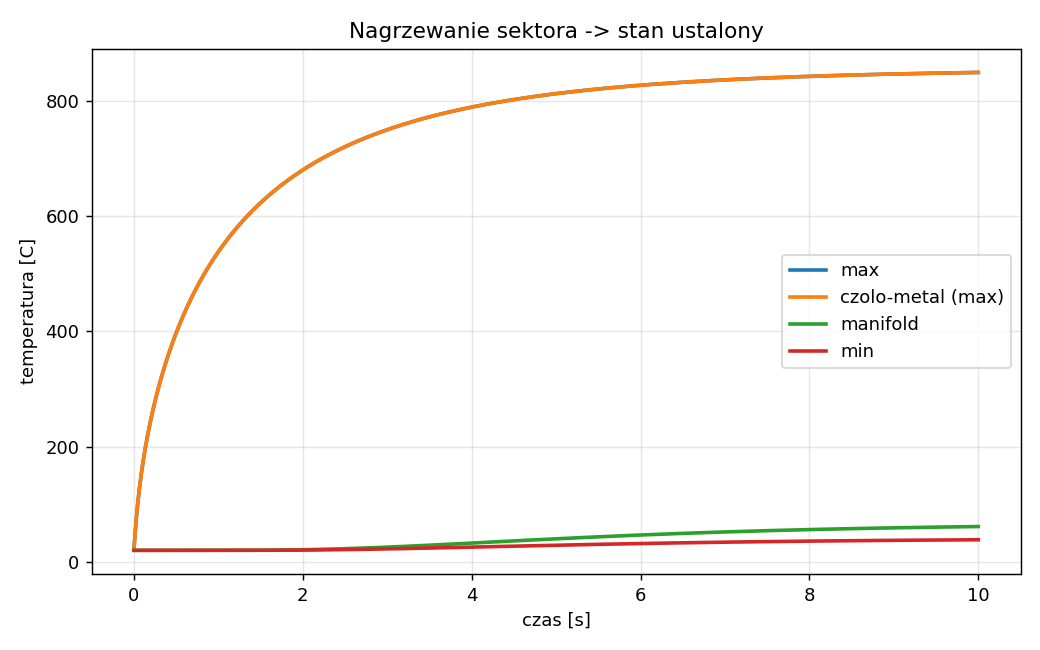
\includegraphics[width=0.72\textwidth]{injector_thermal_transient.png}
\caption{Transient temperature histories of the characteristic probes; the dashed
line marks the whole-body steady-state criterion.}
\label{fig:transient}
\end{figure}

\subsection{Output Parameters}
The key output quantities are summarised in Table~\ref{tab:out}.

\begin{table}[h]
\centering
\caption{Simulation output parameters (316L plate, baseline case).}
\label{tab:out}
\begin{tabular}{lr@{ }l}
\toprule
Parameter & \multicolumn{2}{c}{Value} \\
\midrule
Face metal, maximum (between orifices) & 849.2 & \degC \\
Face metal, minimum (at channel wall)  & 392.6 & \degC \\
In-plane gradient across the face      & 456.6 & K \\
Manifold side (mean)                   & 61.2  & \degC \\
Channel heat-transfer coefficient $h_p$ & 17\,484 & W\,m$^{-2}$K$^{-1}$ \\
Heat removed per orifice               & 157.7 & W \\
HTP bulk temperature rise              & 6.93  & K \\
Heat-up time constant $\tau$           & 1.04  & s \\
\bottomrule
\end{tabular}
\end{table}

% ============================================================
\section{Conclusions}
% ============================================================
A three-dimensional transient finite-volume model of a showerhead injector
operating on hydrogen peroxide was developed and exercised. For the baseline 316L
configuration the simulation predicts:
\begin{enumerate}[noitemsep]
  \item a strongly non-uniform gas-side face temperature, from $\sim\!393\,\degC$
        at the cooled channel wall to $\sim\!849\,\degC$ between orifices
        (a $\sim\!457\,$K in-plane gradient);
  \item a fast thermal response of the critical gas-side face, with a heat-up
        time constant $\tau\approx1.0\,$s;
  \item a manifold side that stays cold ($\sim\!61\,\degC$) thanks to the HTP
        cooling, while the deep through-thickness equilibrium is approached only
        slowly because of the low conductivity of stainless steel.
\end{enumerate}
The framework is fully parametric, so material, mass flow, gas temperature and
geometry can be varied directly in the source code. The largest modelling
uncertainty is the gas-side film coefficient $h_\mathrm{gas}$, to which the
steady-state temperature is nearly proportional; substituting a Bartz-type
correlation or a measured heat flux is the natural next step, together with
temperature-dependent properties and a body-fitted (non-staircase) orifice mesh.

% ============================================================
\begin{thebibliography}{9}
\bibitem{huzel} D.~K.~Huzel and D.~H.~Huang. \emph{Modern Engineering for Design
  of Liquid-Propellant Rocket Engines}. AIAA, 1992.
\bibitem{incropera} F.~P.~Incropera and D.~P.~DeWitt. \emph{Fundamentals of Heat
  and Mass Transfer}. 6th ed., Wiley, 2007.
\bibitem{ventura} M.~Ventura and E.~Wernimont. \emph{History of the Hydrogen
  Peroxide Bipropellant}. AIAA Joint Propulsion Conference, 2007.
\bibitem{sutton} G.~P.~Sutton and O.~Biblarz. \emph{Rocket Propulsion Elements}.
  9th ed., Wiley, 2016.
\end{thebibliography}

\end{document}
